\section{L-systémy}\label{sec:L-systemy}

Uvedeme tuto kapitolu s~ohledem na předchozí obsah trochu netradičně a od matematiky se (alespoň zdánlivě) na chvíli odkloníme. Podíváme se na fraktály,~s jejichž způsobem popisu přišel roku 1968 maďarský biolog \name{Aristid Lindenmayer} (1925--1989) a který (možná pro někoho i~překvapivě) má základy především v~informatice. \citep[str. 2]{Prusinkiewicz1990}

K popisu specifického druhu fraktálů lze využít znalosti z \emph{teorie formálních jazyků} a \emph{teorie automatů}, na jejímž počátku stál (mj.) britský matematik a informatik \name{Alan Turing} (1912--1954). Ten ve svém článku \emph{On Computable Numbers, with an Application to the Entscheidungsproblem} z roku 1936 zavedl koncept abstraktního stroje dnes známého jako \emph{Turingův stroj}\index{Turingův stroj}, jednoduché zařízení s výpočetními schopnostmi již tehdy porovnatelnými se současnými počítači. Jeho princip fungování přitom není nikterak složitý. Pomineme-li nyní matematickou definici Turingova stroje, lze říci, že sestává ze tří hlavních částí:
\begin{enumerate}
    \item \textbf{Oboustranně nekončná páska.} Páska je rozdělena na políčka, z nichž každé může obsahovat některý symbol z z předem známé abecedy (formálně vzato množiny) znaků.
    \item \textbf{Čtecí/zapisovací hlava.} Hlavu si můžeme představit jako čtecí/zapisovací "okénko", které stojí právě nad jedním políčkem pásky. V každém kroku stroj:
    \begin{itemize}
        \item přečte symbol pod hlavou,
        \item podle svého stavu a právě přečteného symbolu rozhodne, jakou akci provést.
    \end{itemize}
    \item \textbf{Řídicí jednotka.} Řídí chování stroje pomocí konečné množiny stavů
    \[Q=\set{q_0,q_1,\ldots,q_n}.\]
    Přechodová funkce $\delta$ pro (ne nutně všechny) dvojice $(\text{stav},\text{znak})$ udává:
    \begin{itemize}
        \item jaký symbol má hlava na pásku zapsat (může přepsat stávající symbol nebo nechat stejný),
        \item do jakého stavu se stroj přepne,
        \item jak se posune hlava: doleva (L), doprava (R) nebo zůstane (N).
    \end{itemize}    
\end{enumerate}
Výpočet pak probíhá takto:
\begin{enumerate}
    \item Stroj začíná ve stavu, který je stanovený jako počáteční. Na pásce je vložen vstup (řetězec symbolů), zbytek pásky je prázdný.
    \item Vždy podle přechodové funkce stroje:
    \begin{itemize}
        \item přečte, co je pod hlavou,
        \item zapíše (případně přepíše) symbol,
        \item přesune hlavu,
        \item přejde do dalšího stavu.
    \end{itemize}
    \item Pokud stroj nemá definovaný přechod pro aktuální stav a symbol na pásce, zastaví se. Pokud stroj skončil ve stavu, který je označený jako přijímající, pak stroj slovo \textbf{přijal}, jinak jej \textbf{odmítá}.
\end{enumerate}
\begin{figure}[h]
    \centering
    \begin{tikzpicture}[>=Stealth, every node/.style={font=\sffamily},
        box/.style={rectangle, draw=black, rounded corners, fill=yellow!30, inner sep=8pt},
        smallbox/.style={rectangle, draw=black, fill=yellow!10, inner sep=4pt, minimum width=1cm, minimum height=1cm},
        tapecell/.style={rectangle, draw=black, fill=yellow!10, minimum size=0.8cm},
        head/.style={isosceles triangle, draw=black, fill=gray!30, shape border rotate=180, minimum width=0.8cm, minimum height=0.6cm},
        callout/.style={draw=teal!80!black, fill=teal!20, rounded corners, font=\sffamily\small}
      ]
      % Control unit
      \node[box] (ctrl) {\textbf{Řídící jednotka}
        \begin{tikzpicture}[baseline]
          \node[smallbox] (delta) {$\delta$};
          \node[smallbox, right=1em of delta] (q) {$q$};
        \end{tikzpicture}
      };
      % Transition function label
      \node[callout, callout relative pointer={(0.5cm,-0.5cm)}] at (ctrl.west) {Přechodová funkce};
      % Current state label
      \node[callout, callout relative pointer={(-0.5cm,-0.5cm)}] at (ctrl.east) {Aktuální stav};
      
      % Head arrow
      \node[head, below=2cm of ctrl] (head) {};
      % Head movement arrows
      \draw[<->] (head.east|-head) -- ++(1cm,0) node[midway, above] {};
      \draw[<->] (head.west|-head) -- ++(-1cm,0) node[midway, above] {};
      % Head label
      \node[callout, callout relative pointer={(0,-0.5cm)}] at (head.north) {Čtecí a zapisovací hlava, která se může pohybovat oběma směry};
      
      % Tape cells
      \matrix (tape) [matrix of nodes, nodes={tapecell}, row sep=0mm, column sep=0mm, below=1.5cm of head] {
        $\dots$ & H & e & l & l & o & \_ & w & o & r & l & d & $\dots$ \\
      };
      % Tape annotations
      \node[below=2mm of tape] {Neomezená páska};
      \node[callout, callout relative pointer={(0,0.8cm)}] at (tape-1-7.south) {Prázdné políčko};
      \node[callout, callout relative pointer={(0,0cm)}] at (tape-1-9.east) {Symboly páskové abecedy};
      
    \end{tikzpicture}
    \caption{Znázornění Turingova stroje}
    \label{fig:turinguv-stroj}
\end{figure}
\begin{figure}[h]
    \centering
    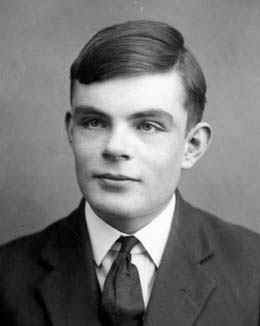
\includegraphics[width=.4\textwidth]{Alan-Turing.jpeg}
    \caption[Alan Turing,~1871--1956]{Alan Turing\footnote{Převzato z~\cite{OConnorTuring2025}},~1912--1954}
    \label{fig:alan-turing}
\end{figure}
V té době se zabýval otázkou, kterou v roce 1928 položil známý německý matematik \name{David Hilbert} (1862--1943), jež je známá pod názvem \emph{"Entscheidungsproblem"}\index{Entscheidungsproblem}\footnote{Anglicky \emph{The Decision problem}\index{The Decision problem}, česky přeložitelné jako \emph{"rozhodovací problém"}. Zde však poznamenejme, že onem český termín se používá i v související teorii složitosti a vyčíslitelnosti, má však podstatně jiný význam.}. Problémem bylo, zda existuje algoritmus, který o každém tvrzení je schopný rozhodnout (v konečném čase), zda je či není pravdivé. Později Alan Turing tento problém přeformuloval takto: \emph{Existuje program, který o jiném programu na vstupu rozhodne, zda se zastaví, či nikoliv?} David Hilbert byl ve svých vizích optimistický, avšak nakonec Alan Turing dokázal, že \textbf{takový algoritmus nemůže existovat}. Způsob, jakým Turing došel onomu výsledku, byl v konečném důsledku vlastně až překvapivě jednoduchý a existuje pro něj velké množství popularizačních materiálů\footnote{Pokud by se chtěl čtenář dozvědět více o této problematice a teorii s ní související, doporučuji např. knihu \cite{Motwani2003}}.
\begin{figure}[h]
    \centering
    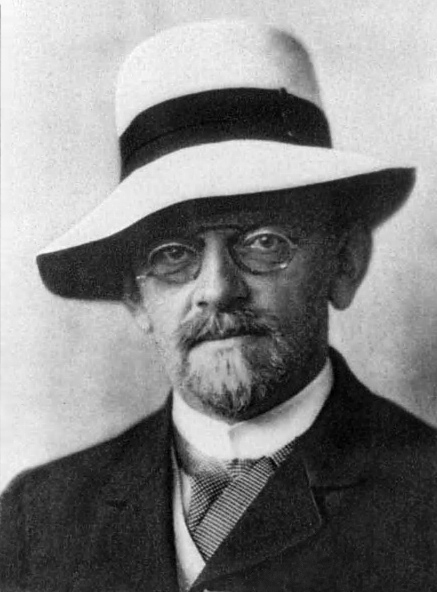
\includegraphics[width=.4\textwidth]{David-Hilbert.jpg}
    \caption[David Hilbert,~1862--1943]{David Hilbert\footnote{Převzato z~\cite{OConnorHilbert2025}},~1862--1943}
    \label{fig:david-hilbert}
\end{figure}
Alan Turing dal základ dnešní teoretické informatice. Turingův stroj, co by výpočetní model, stojí na samotném vrchlu hierarchie dalších výpočetních modelů\footnote{Mezi ně patří jmenovitě tzv. \textit{lineárně omezený automat}\index{automat!lineárně omezený}, \emph{zásobníkový automat}\index{automat!zásobníkový}, \emph{deterministický}\index{automat!deterministický} a \emph{nedeterministický konečný automat}\index{automat!nedeterministický}.}, které jsou však svoji výpočetní silou slabší.  Později pak americký matematik \name{Noam Chomsky} (1928--současnost) popsal celkem 4 základní třídy tzv. \emph{formálních jazyků}, které jsou dnes souhrně známé pod názvem \emph{Chomského hierarchie}\index{Chomského hierarchie}. Za formální jazyk považujeme určitou množinu slov (rětězců). Chomského hierarchie zařazuje každý jazyk do jedné ze tříd podle výpočetního modelu, který jej přijímá, resp. typu tzv. \emph{formální gramatiky}, která slova z něj generuje. O gramatikách a obecně určitém základu teorie formálních jazyků si ještě budeme podrobněji povídat později. O hlubší související teorii se čtenář může více dozvědět např. v knize \cite{Motwani2003}.

\subsection{Odbočka k formálním jazykům a gramatikám}\label{subsec:formalni-jazyky-a-gramatiky}

V úvodu této sekce jsme si již trochu přiblížili historické pozadí teorie formálních jazyků a automatů (tou se již dále zabývat nebudeme, nicméně bylo by při nejmenším neslušné ji zde alespoň nezmínit vzhledem k její přímé souvislosti). Ačkoliv tento text si neklade za cíl seznámit čtenáře se všemi podrobnostmi, byly zmíněny určité termíny, jejichž význam bude dobré si objasnit, konkrétně
\begin{itemize}
    \item \emph{formální jazyk}\index{formální!jazyk}\index{jazyk}
    \item a \emph{formální gramatika}.\index{formální!gramatika}\index{gramatika}
\end{itemize}
\begin{definition}\label{def:formalni-jazyk-etc}
    Množinu symbolů (znaků)\index{symbol}\index{znak} $\Sigma$ nazýváme \emph{abeceda}\index{abeceda}.
    \begin{itemize}
        \item Libovolnou konečnou posloupnost znaků
        \[w=a_1a_2\ldots a_n,\]
        kde $a_i\in\Sigma$ pro každé $1\leqslant i\leqslant n$ nazýváme \emph{slovo}\index{slovo}
        \item Prázdným slovem\index{prázdné slovo} nazýváme slovo neobsahující žádné znaky, značíme $\lambda$.
        \item Délku slova\index{délka slova} $w$ značíme $|w|$, tzn.
        \[|w|=|a_1a_2\ldots a_n|=n.\]
        \item Množinu všech slov délky $n$ značíme $\Sigma^n$, tj.
        \[\Sigma^n=\set{a_1a_2\ldots a_n\mid a_i\in\Sigma\;\text{pro každé $i\in\N$}}.\]
        Speciálně $\Sigma^0=\set{\lambda}$.
        \item Množinu všech slov v abecedě $\Sigma$ značíme $\Sigma^*$, tzn.
        \[\Sigma^*=\bigcup_{n=1}^\infty\Sigma^n.\]
        \item Množinu všech neprázdných slov v abecedě $\Sigma$ značíme $\Sigma^+$, tzn.
        \[\Sigma^+=\Sigma^*\setminus\set{\lambda}.\]
        \item \emph{Formálním jazykem} (nebo zkráceně jen \emph{jazykem})\index{formální!jazyk}\index{jazyk} nazýváme libovolnou podmnožinu $L\subseteq\Sigma^*$.
    \end{itemize}
\end{definition}
\begin{example}
    Některé příklady abeced:
    \begin{itemize}
        \item $\Sigma=\set{0,1}$, tzv. \emph{binární abeceda}.
        \[\set{0,1}^*=\set{\lambda,0,1,00,01,10,11,000,001,\ldots}\]
        \item $\Sigma=\set{a,b,c,\ldots,z}$, tj. všechna písmena anglické abecedy.
        \[\set{a,b,c,\ldots,z}^*=\set{a,b,c,\ldots,z,aa,ab,ac,\ldots}\]
        \item Všechny znaky ASCII\footnote{Zkratka pro \emph{American Standard For Information Interchange}. Stanovuje 128-bitové znakové kódování. Podoktněme, že ne všechny znaky jsou nutně tisknutelné a mají čistě informativní charakter, avšak to nás zde z formálního hladiska trápit vůbec nemusí.} tvoří abecedu.
    \end{itemize}
\end{example}
\begin{definition}[Operace se slovy]\label{def:operace-se-slovy}
    Nechť $\Sigma$ je libovolná abeceda a mějme slova $u,v\in\Sigma^*$, kde $u=u_1u_2\ldots u_n$ a $v=v_1v_2\ldots v_m$. Pak definujeme následující operace:
    \begin{itemize}
        \item \emph{Zřetězení (konkantenace)}\index{zřetězení}\index{konkantenace} slov $u$ a $v$ je slovo
        \[uv=u_1u_2\ldots u_nv_1v_2\ldots v_m.\]
        Je celkem zjevné, že $|uv|=|u|+|v|=n+m$.
        \item Nechť $n\in\N$. Pak definujeme induktivně:
        \begin{align*}
            u^0&=\lambda,\\
            u^1&=u,\\
            u^n&=u^{n-1}u.
        \end{align*}
        Slovo $u^n$ se nazývá \emph{$n$-tá mocnina slova}\index{mocnina slova} $u$.
        \item \emph{Obráceným slovem $u$} rozumíme slovo $u^R=u_nu_{n-1}\ldots u_1$.
    \end{itemize}
\end{definition}
\begin{remark}
    Speciálně pro prázdné slovo $\lambda$ a libovolné slovo $u\in\Sigma^*$ platí $u\lambda=\lambda u=u$.
\end{remark}
Na základě definice \ref{def:operace-se-slovy} můžeme být nyní daleko konkrétnější při popisu některých slov a jazyků. Např.
\[L=\set{0^n1^n\mid n\in\N}\]
značí jazyk všech slov obsahující znaky $0$ a $1$ ve tvaru
\[\lambda,01,0011,000111,\ldots\]
O jazycích celkově lze dokázat řadu zajímavých tvrzení, která se přímo opírají o již zmínenou teorii automatů. V tomto ohledu si dovolíme však hodně záležitostí přeskočit. Jazyky lze popisovat několika různými způsoby, avšak nás bude zajímat popis pomocí formálních gramatik\index{formální!gramatika}\index{gramatika}.
\begin{definition}[Formální gramatika]\label{def:formalni-gramatika}
    \emph{Formální gramatikou} (zkráceně jen gramatikou \emph{gramatikou})\index{formální!gramatika}\index{gramatika} nazýváme uspořádanou čtveřici $G=(V,T,P,S)$, kde
    \begin{itemize}
        \item $V\neq\emptyset$ je množina \emph{neterminálů}\footnote{Anglicky \emph{variables}}\index{neterminál} (neterminálních symbolů)\index{neterminální symbol},
        \item $T\neq\emptyset$ je množina \emph{terminálů}\index{terminál} (terminálních symbolů)\index{terminální symbol},
        \item $S\in V$ je \emph{počáteční symbol},
        \item a $P$ je množina přepisovacích \emph{pravidel}\footnote{Formálně vzato se jedná o uspořádanou dvojici $(\alpha,\omega)$.}\index{přepisovací pravidlo}\index{pravidlo} ve tvaru $\beta A\gamma\to\omega$ (čteme "řetězec $\beta A\gamma$ se přepíše na řetezec $\omega$"), kde $A\in T$ a $\beta,\gamma,\omega\in(V\cup T)^*$. Tzn. levá strana každého pravidla obsahuje alespoň jeden neterminál.
    \end{itemize}
\end{definition}
\begin{definition}[Odvození slova]\label{def:odvozeni-slova}
    Mějme gramatiku $G=(V,T,P,S)$. Říkáme, že
    \begin{itemize}
        \item $\alpha$ se \emph{přímo přepíše} na $\omega$, píšeme $\alpha\Rightarrow_G\omega$ nebo jen $\alpha\Rightarrow\omega$, jestliže
        \[\exists\beta,\gamma,\eta,\nu\in(V\cup T)^*: \alpha=\eta\beta\nu,\omega=\eta\gamma\nu\land(\beta\to\gamma)\in P.\]
        \item $\alpha$ se \emph{přepíše} na $\omega$, píšeme $\alpha\Rightarrow_G^*\omega$ nebo jen $\alpha\Rightarrow^*\omega$, pokud
        \[\exists\beta_1,\beta_2,\ldots,\beta_n\in(V\cup T)^*:\alpha=\beta_1\Rightarrow\beta_2\Rightarrow\dots\Rightarrow\beta_n=\omega.\]
    \end{itemize}
    Posloupnost $\beta_1,\ldots,\beta_n$ nazýváme odvozením\index{odvození slova}. Též říkáme, že gramatika $G$ generuje slovo $w$, pokud $S\Rightarrow^* w$.
\end{definition}
Formální gramatiky nám umožňují rekurzivní definici jazyka. Jinak řečeno, popisuje, jak lze slova daného jazyka generovat. Pravidla z množiny $P$ lze aplikovat v libovolném pořadí.
\begin{remark}
    \begin{itemize}
        \item Typicky platí, že pro neterminály používáme velká písmena abecedy $A,B,\ldots,Z$ a pro terminály naopak malá písmena $a,b,\ldots,z$, popř. i jiné symboly.
        \item Pokud máme více pravidel ve tvaru $\alpha\to\omega_i$, tj. se shodnou levou stranou, pak pro jejich zápis volíme tuto kompaktnější variantu:
        \[\alpha\to\omega_1\mid\omega_2\mid\dots\mid\omega_n.\]
    \end{itemize}
\end{remark}
\begin{example}
    Jazyk všech palindromů nad binární abecedou, tj.
    \[L_\text{pal}=\set{w\in\set{0,1}^*\mid w=w^R}.\]
    lze generovat gramatikou $G=\set{\set{S},\set{0,1},P,S}$, přičemž $P$ obsahuje následující pravidla:
    \[S\to\lambda\mid 0\mid 1\mid 0S0\mid 1S1.\]
    Kupříkladu slovo $w=011110$ lze odvodit takto:
    \[S\Rightarrow 0S0\Rightarrow 01S10\Rightarrow011S110\Rightarrow011\lambda 110=011110.\]
\end{example}
Trochu praktičtěji zaměřený příklad nám poskytuje \ref{ex:syntax-analyza}. Gramatiky se typicky využívají (vyjma fraktální geometrie) např. v kompilátorech\index{kompilátor} různých programovacích jazyků v rámci tzv. \emph{syntaktické analýzy}\index{syntaktická analýza}, při níž se (jak název napovídá) kontroluje syntaktická správnost zápisu programu. Konkrétně se pro jednoduchost zaměříme pouze na matematické výrazy obsahující pouze operace \texttt{+} a \texttt{*} (násobení).
\begin{example}\label{ex:syntax-analyza}
    Mějme gramatiku $G=(V,T,P,S)$, kde
    \[V=\set{E,I},T=\set{a,b,(,),+,*},S=E\]
    a pravidla jsou následující:
    \begin{align*}
        E&\to I\mid E+E\mid E*E\mid (E)\\
        I&\to a\mid b\mid Ia\mid Ib.
    \end{align*}
    V takto definované gramatice lze vygenerovat např. slovo
    \[w=(a+b)+bb*(ab+bb)\]
    následovně:
    \begin{align*}
        E&\Rightarrow E+E\Rightarrow(E)+E\Rightarrow(E)+E*E\Rightarrow(E)+E*(E)\\
        &\Rightarrow(E+E)+E*(E)\Rightarrow(E+E)+E*(E+E)\\
        &\Rightarrow^*(I+I)+I*(I+I)\Rightarrow^*(a+b)+Ib*(Ib+Ib)\\
        &\Rightarrow^*(a+b)+bb*(ab+bb).
    \end{align*}
\end{example}
S podobným přístupem se lze setkat i např. v lingvistice. Čtenář si možná ze základní školy větný rozbor, v jehož rámci bylo úkolem určit pro zadanou větu její strukturu. Ve skutečnosti se nejedná o nic jiného, než využítí určité formální gramatiky $G=(V,T,P,S)$, jejíž pravidla v množině $P$ jsou dána gramatickými pravidly (nyní v lingvistickém slova smyslu) českého jazyka. Pro příklad viz obrázek\footnote{S, NP, VP, ADJP představují neterminály příslušné gramatiky a jednotlivá slova (Petr, četl, pěknou, knihu) její termínály. Významy: S \emph{(Sentence)}, NP \emph{(Noun Phrase)}, VP \emph{(Verb Phrase)}, ADJP \emph{(Adjective Phrase)}.} \ref{fig:syntax-strom-vety}.
\begin{figure}[h]
    \centering
    \begin{tikzpicture}[
        edge from parent/.style={draw, -latex},
        level distance=1.5cm,
        sibling distance=3cm
      ]
        \node {S}
          child { node {NP}
            child { node {Petr} }
          }
          child { node {VP}
            child { node {\textit{četl}} }
            child { node {NP}
              child { node {ADJP}
                child { node {\textit{pěknou}} }
              }
              child { node {knihu} }
            }
          };
    \end{tikzpicture}
    \caption{Příklad syntaktického stromu věty: \emph{"Petr četl pěknou knihu."}}
    \label{fig:syntax-strom-vety}
\end{figure}
Zároveň zde můžeme vidět souvislost formální gramatiky s gramatikou v lingvistice.

\subsection{Definice L-systému}\label{subsec:definice-lsystemu}

V podsekci \ref{subsec:formalni-jazyky-a-gramatiky} jsme si udělali v podstatě "rychloúvod" do problematiky \emph{formálních jazyků} a \emph{gramatik}, kde jsme si především zavedli potřebné značenou terminologii a značení. L-systémy se v kontextu formálních gramatik mírně, avšak podstatně liší v tom, že pravidla jsou v jednom kroku aplikována paralelně. 